% Gabriel

\subsubsection*{Principe de la méthode} 

Cette méthode part du constat suivant : les facettes colorées du cube sont séparées par une zone nettement plus sombre. Cette zone se caractérise par l'apparition de pics sur les projections en abscisses et ordonnées. 

Dans un premiers temps nous avons fixé manuellement un seuil pour délimiter les facettes colorées. Nous nous sommes rapidement rendus comte que le seuil fixe ne pouvait convenir à des images dont les conditions d'éclairage varient. 

Nous avons donc réalisé un algorithme de détection de seuil dont le principe est le suivant : Nous commençons par fixer un seuil à la valeur la plus sombre de la projection.

Ensuite nous éclairsissons la valeur de ce seuil jusqu'à croiser un minimum de deux pics distincts.

\subsubsection*{Résultats obtenus par cette méthode}
 
 Nous réalisons par exemple un seuillage sur la courbe suivante (figure \ref{projX}):
 \begin{figure}[!h]
 \centering
 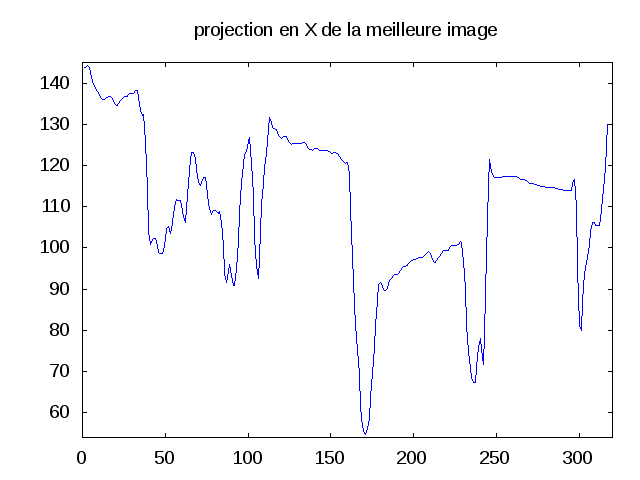
\includegraphics[width=0.60\linewidth]{Images/projX.png}
 \caption{projetée en abscisses} 
 \label{projX}
 \end{figure}
 
 Nous pouvons notament obtenir le résultat suivant (figure \ref{barreGlissante}):
\begin{figure}[!h]
 \centering
 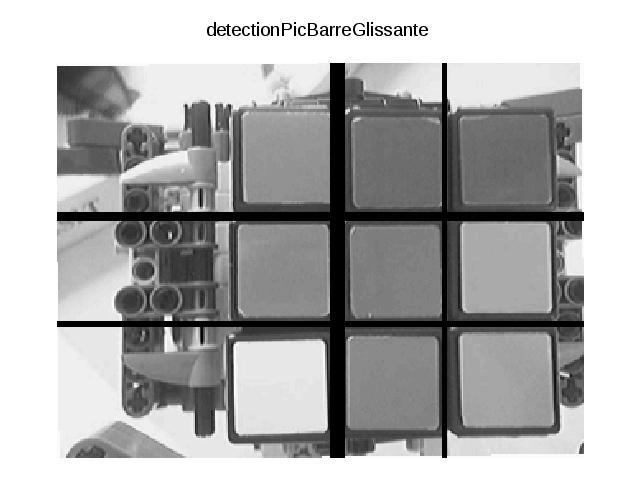
\includegraphics[width=0.60\linewidth]{Images/detectionBarreGlissante.png}
 \caption{détéction par la méthode de la barre de seuillage} 
 \label{barreGlissante}
 \end{figure}
